\chapter{人和物体交互静态重建}\label{chap:stackflow}
对人和物体之间的三维空间关系建模是从单张图片中感知人和物体之间交互的关键,本章提出使用人-物偏移量来对人和物体之间的三维空间关系进行表征(章节\ref{sec:offset-representation}),和之前基于接触面的表征或者基于隐式场的表征相比,本章所提出的表征方法能够更加简洁、高效、细粒度的表示人和物体之间的三维空间关系。基于该偏移量的表征方式,本章进一步提出了叠层归一化流模型从单视角图片中提取人和物体之间的空间关系的后验概率密度分布,在后优化过程中通过最大化人-物空间关系的后验概率和最小化人-物的重投影损失来微调结果(章节\ref{sec:stackflow})。最后,本章在BEHAVE数据集中和其他方法进行了定性和定量的对比,结果表明本章所提出的方法具有更高的运行效率和重建精度,尤其是在人和物体严重遮挡的情况下表现优异(章节\ref{sec:exp-stackflow})。

\section{人和物体三维表征}\label{sec:offset-representation}
\subsection{人体三维表征}
本文使用SMPL模型
%\footnote{本文侧重于人体和物体之间的交互,而不涉及人手和物体之间的交互,为了和数据集或其它算法兼容,后续虽使用到SMPL-H或SMPL-X模型,但没有对人手姿态做出算法上特定的设计。}
来参数化表示三维人体结构。SMPL模型\citep{SMPL}是一种在学术界广泛使用的人体三维结构参数化模型,在SMPL模型中,人体的三维结构由三维网格模型$\mathcal{M}^{\text{h}}=(\mathbf{V}^{\text{h}},  \mathbf{F}^{\text{h}})$所表示,其中$\mathbf{V}^{\text{h}} \in \mathbb{R}^{6890 \times 3}$是该网格模型的点集,$\mathbf{F}^{\text{h}} \in \mathbb{R}^{13776 \times 3}$是面集,每一个面定义了点的连接关系。在SMPL模型的局部坐标系下,顶点的三维坐标由形状参数$\mathbf{\beta} \in \mathbb{R}^{10}$和姿态参数$\mathbf{\theta} \in \mathbb{R}^{69}$所决定,即
\begin{equation}\label{eq:smpl-blending}
	\mathbf{V}^{\text{h}} = \mathcal{B}(\mathbf{\beta}, \mathbf{\theta}),
\end{equation}
式中,$\mathcal{B}$是线性蒙皮函数(linear  blend skinning function),它建立起从形状参数$\mathbf{\beta}$和姿态参数$\mathbf{\theta}$到顶点坐标$\mathbf{V}^{\text{h}}$之间的映射。人体各个关节节点的三维坐标$\mathbf{J} \in \mathbb{R}^{22 \times 3}$可以从网格模型的顶点坐标获得,两者之间的关系如下:
\begin{equation}
	\mathbf{J} = \mathbf{W} \mathbf{V}^{\text{h}},
\end{equation}
式中,$\mathbf{W} \in \mathbb{R}^{22 \times 6890}$是权重矩阵,它衡量网格模型中顶点对人体关节节点的贡献程度。

\subsection{物体三维表征}
相比于人体结构,物体形态是极为丰富,对物体的建模涉及复杂的拓扑和几何关系,不属于本章所研究的范畴。本文假设物体的拓扑几何关系已知,并被表示成三维网格模型$\mathcal{M}^{\text{o}} = (\hat{\mathbf{V}}^{\text{o}}, \mathbf{F}^{\text{o}})$,其中$\hat{\mathbf{V}}^{\text{o}}$是在物体网格模型局部坐标系下的顶点坐标,$\mathbf{F}^{\text{o}}$规定这些顶点如何相连形成面。这些网格模型的获得可以通过以下三种途径:(1)使用高精度扫描仪扫描特定物体,(2)从CAD模型库内人工挑选出符合目标物体的三维网格模型,(3)使用重建算法\citep{BundleSDF}从输入源中自适应重建物体。在实际应用中,会根据不同的需求选取不同的途径来获取物体的先验网格模型。

\subsection{人-物三维空间关系表征}
人在三维空间中通过不同的方式与物体发生交互,在每一种交互方式中,人和物体存在特定的空间位置关系,称在该特定空间位置关系下的人和物体为一个人-物交互实例(HOI instance)。在人体SMPL模型局部坐标系下,每一个人-物交互实例$(\mathcal{M}^{\text{h}},\mathcal{M}^{\text{o}})$可使用参数$\{\mathbf{\beta}, \mathbf{\theta}, \mathbf{R}, \mathbf{t}\}$来刻画,其中,人体模型顶点的位置由${\mathbf{\beta}, \mathbf{\theta}}$通过式(\ref{eq:smpl-blending})确定,而物体模型顶点的位置通过物体相对于人体的位姿确定,即物体模型中每一个顶点空间坐标的计算方式为
\begin{equation}
	\mathbf{V}^{\text{o}}_i = \mathbf{R} \hat{\mathbf{V}}^{\text{o}}_i + \mathbf{t},
\end{equation}
式中,$\mathbf{R}\in\mathbb{R}^{3\times 3}$和$\mathbf{t}\in\mathbf{R}^3$分别为物体在SMPL模型局部坐标系下的旋转矩阵和平移向量。在以$\{\mathbf{\beta}, \mathbf{\theta}, \mathbf{R}, \mathbf{t}\}$为参数的人-物交互刻画的方式中,人和物体分别被不同的参数决定,这种表示方式无法有机融合两者,为了进一步对人和物体之间的空间关系进行约束,先前方法采用了基于接触面的方法和基于隐式向量场的方法。在基于接触面的方法中,接触面被定义为人体网格模型和物体网格模型中相接触的区域,在后优化过程中通过将人体和物体网格模型中的接触点拉近来生成合理的结果。然而接触面只保留了局部接触的信息,无法刻画一些非接触的交互类型,此外,它依赖于人体和物体合理的初始化位姿,因此它不是一种独立的对人体-物体空间关系编码的方式。另外一种刻画人体和物体之间空间关系的方法使用了隐式向量场,它定义了一个3D点到点-面最近距离的映射函数,这种方法适用于建模三维物体的形状,但在建模人体-物体之间的空间关系会出现一些缺陷,首先,为了还原出人和物体之间的空间关系,需要在空间中采样很多点来逼近表面,这在后优化中是一种低效的方式。此外,使用函数化的表达而不是向量化的表达会导致将概率模型应用到对人-物空间关系建模上是困难且间接的。为了追寻一种全局的、独立的、向量化的、高效的对人体和物体空间关系统一的刻画方式,本文提出了基于偏移量的表示。

\begin{figure}[!htbp]
	\centering
	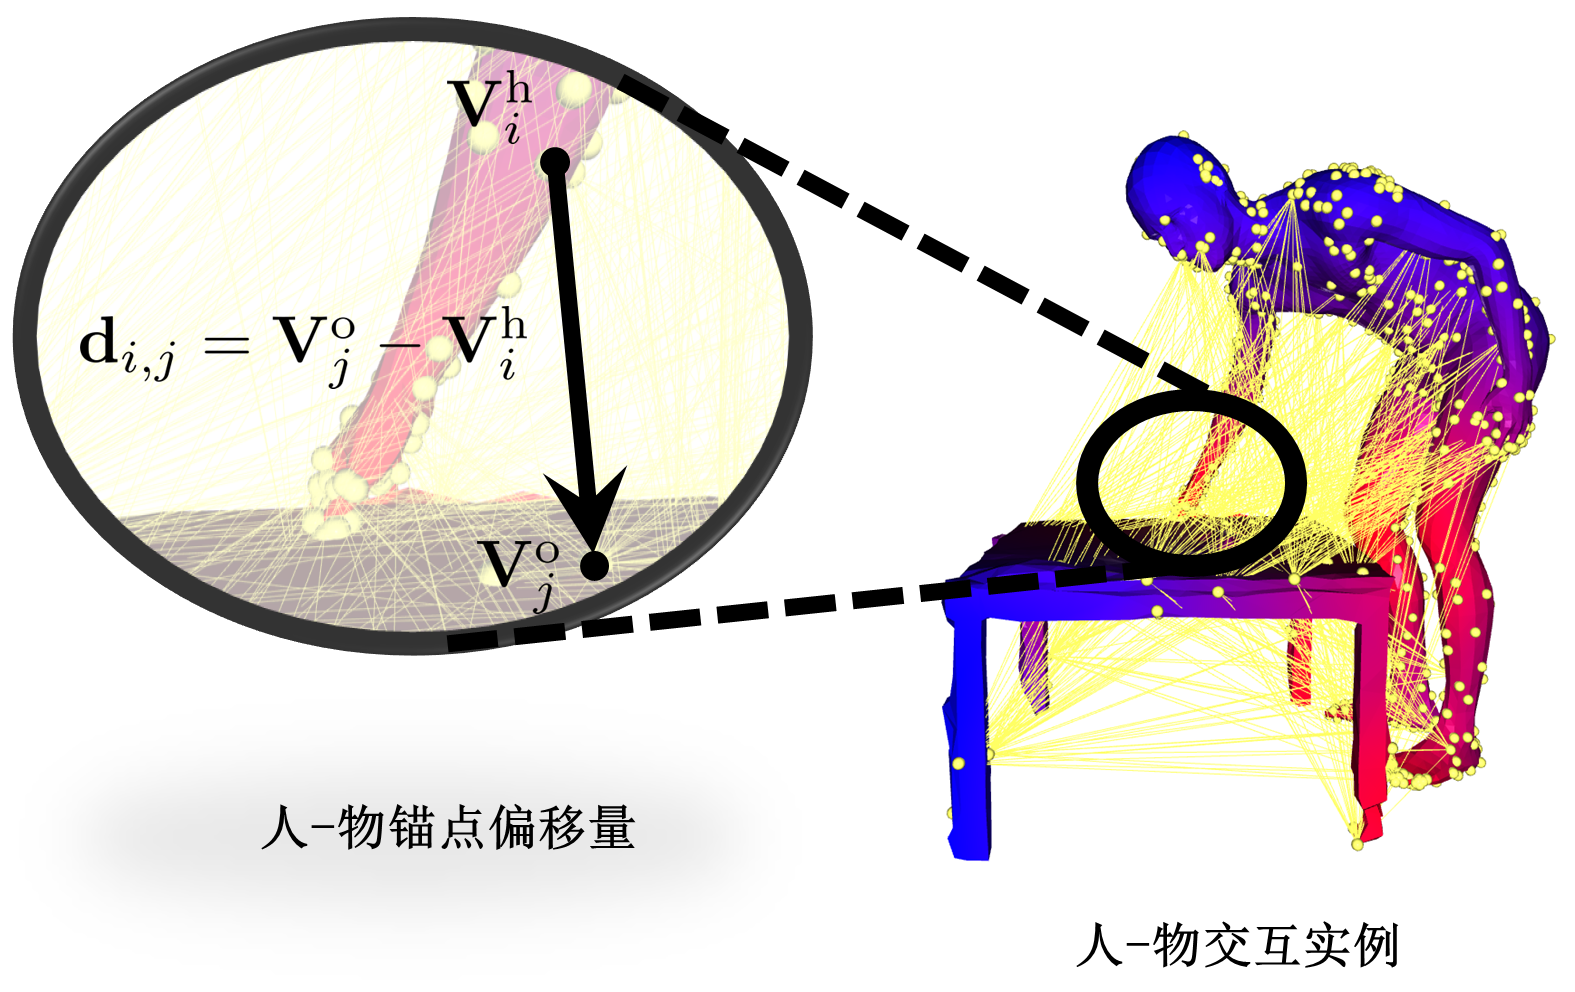
\includegraphics{Img/ho_offsets}
	\bicaption{人和物体之间的偏移量。}{The offsets between the human and the object.}
	\label{fig:offset}
\end{figure}

如图\ref{fig:offset}所示,在基于偏移量的表示中,人-物交互实例由人体和物体网格模型表面的锚点之间的偏移量所刻画,这些偏移量控制着人和物体之间的相对距离,人和物体被有机地结合在一起,相互影响。具体而言,首先,分别从给定的人体三维网格模型和物体三维网格模型中随机均匀地采样出$m$个点和$n$个点,以形成人体锚点的索引集合$\mathcal{A}_{\text{h}} = \{ i_1^\text{h}, i_2^\text{h}, \dots, i_m^\text{h} \}$和物体锚点的索引集合$\mathcal{A}_{\text{o}} = \{ i_1^\text{o}, i_2^\text{o}, \dots, i_n^\text{o} \}$,集合中任意元素$i$表示物体网格模型或者人体网格模型中的第$i$个顶点的索引。对于人和同一种物体网格模型的交互,所有人-物交互实例共享同一组锚点索引,这些锚点索引预先选取且在表征过程中保持不变。对于任意一对人和物体交互的实例,最一般的刻画方式使用$\mathbf{\beta}$和$\mathbf{\theta}$来刻画人体形状和姿态,使用$\mathbf{R}$和$\mathbf{t}$来刻画物体相对于物体的位姿,而在基于偏移量的表示形式下,人和物体之间的空间关系由一组偏移量表示,其中每一个偏移量由下式计算,
\begin{equation}\label{eq:offset}
	\mathbf{d}_{i,j} = \mathbf{V}_{j}^{\text{o}} - \mathbf{V}_{i}^{\text{h}}, i \in \mathcal{A}_{\text{h}}, j \in \mathcal{A}_{o},
\end{equation}
其中,$\mathbf{d}_{i,j}$表示在SMPL模型局部坐标系统下人体网格模型中第$i$个顶点$\mathbf{V}_{i}^{\text{h}}$和物体网格模型中第$j$个顶点$\mathbf{V}_{j}^{\text{o}}$之间的偏移向量。将所有的偏移量相连接形成一个总偏移向量$\mathbf{x}\in \mathbb{R}^{3mn}$,该偏移向量是对人和物体之间的三维空间关系的一种刻画。在原本最一般化的表示中,人和物体被四个参数$\{\mathbf{\beta}, \mathbf{\theta}, \mathbf{R},\mathbf{t}\}$来表示,其中存在85(10+69+3+3)个自由度,然而在基于偏移量的表示下,向量的维度为$3mn$,对于较大的$m$或$n$,这种表示方式会存在信息冗余的问题。

为了得到对人和物体空间关系更加紧凑的编码方式,本文采用主成分分析来对偏移向量进行降维。对训练集合中所有的人和物体关系计算上述的偏移向量,将这些偏移向量相连接在一起形成矩阵$\mathbf{X}\in \mathbb{R}^{t\times 3mn}$,其中$t$为偏移向量的个数。使用主成分分析提取矩阵$\mathbf{X}$前$k$个主成分向量,这些主成分向量相互正交,构成了人和物体偏移量的隐空间的基向量。给定任意一组偏移向量$\mathbf{x}$,它可以通过下式投影在该隐空间内,
\begin{equation}
	\mathbf{\gamma} = \mathbf{P}^T(\mathbf{x} - \mathbf{\mu}),
\end{equation}
式中,$\mathbf{P}\in \mathbb{R}^{3mn\times k}$是由前$k$个主成分向量构成的投影矩阵,$\mathbf{\mu}$是偏移向量$\mathbf{x}$的均值向量,$\mathbf{\gamma} \in \mathbb{R}^{k}$为该偏移向量$\mathbf{x}$投影在该隐式人-物关系空间内的隐向量。最终,人和物体在三维空间中的空间关系被编码成隐式向量$\mathbf{\gamma}$。

一种好的表征除了满足数据紧凑性之外,还需满足信息完整性,基于偏移量的表征方式不仅仅编码了人和物体之间的三维空间关系,还提供了对人体姿态和物体位姿的约束。给定人和物体三维空间关系的隐式表达$\mathbf{\gamma}$,通过逆向投影得到人体和物体之间的偏移量,即
\begin{equation}\label{eq:reproject-offset}
	\hat{\mathbf{x}} = \mathbf{P}\mathbf{\gamma} + \mathbf{\mu}.
\end{equation}
人体位姿$\mathbf{\beta},\mathbf{\theta}$和物体位姿$\mathbf{R},\mathbf{t}$可以通过调整人体锚点和物体锚点之间的偏移量从$\hat{\mathbf{x}}$重构出,即
\begin{equation}\label{eq:recon_from_offset}
	\{\hat{\mathbf{\beta}}, \hat{\mathbf{\theta}}, \hat{R}, \hat{\mathbf{t}} \} = \mathop{\arg\min}\limits_{\mathbf{\beta}, \mathbf{\theta}, \mathbf{R}, \mathbf{t}} \sum_{i \in \mathcal{A}_{\text{h}}} \sum_{j \in \mathcal{A}_{\text{o}}} \| \mathbf{V}_i^{\text{h}} + \hat{\mathbf{d}}_{i,j} - \mathbf{V}_j^\text{o} \|^2.
\end{equation}
上式中,$\{\hat{\mathbf{\beta}}, \hat{\mathbf{\theta}}, \hat{R}, \hat{\mathbf{t}}\}$是从偏移向量$\hat{\mathbf{x}}$重构出的人体位姿和物体中位姿,$\hat{\mathbf{d}}_{i,j}$取自$\hat{\mathbf{x}}$对应位置的元素。

\section{基于叠层归一化流的重建算法}\label{sec:stackflow}
为了从输入图片$\mathbf{I}$重构出以偏移量为表征的人和物体之间的空间关系,本节提出了一种基于叠层归一化流的重建算法。如图\ref{fig:stackflow}所示,该重建算法采用预测-优化的两阶段框架,在预测阶段,使用叠层归一化流提取图片中人和物体之间的三维空间关系的后验分布$p_{\Gamma|I}(\mathbf{\gamma}|\mathbf{c})$,在联合优化阶段微调预测的结果,通过重投影损失将重建的结果和图片的关键点保持对齐。

\subsection{叠层归一化流}
由于单视角三维重建自身存在的自遮挡和人-物相互遮挡的情况,直接从输入图片确定性回归人和物体的空间关系编码是充满歧义性的,本文采用归一化流的概率化刻画方式。给定图片$\mathbf{I}$,归一化流模型(StackFLOW)从图片中提取人和物体空间关系$\mathbf{\gamma}$的概率密度分布$p_{\Gamma|\mathcal{I}}(\mathbf{\gamma}|\mathbf{c})$,其中$\mathbf{c}$是从输入图片$\mathbf{I}$提取的视觉特征,该条件概率密度分布建立起从图像空间$\mathcal{I}$到人-物关系空间$\mathcal{\Gamma}$之间的对应关系,即给定从图像空间$\mathcal{I}$中任一图片$I$提取的视觉特征$\mathbf{c}$,该条件分布给出该图片中人和物体空间关系在空间$\mathcal{\Gamma}$中的概率密度。然而,在实践中,模型是很难从输入图片中直接学习到人-物空间关系$\mathbf{\gamma}$的概率分布。为了缓解模型的训练过程,本文采用了叠层归一化流的设计,将空间关系的概率密度分布拆分成两个条件分布,即
\begin{equation}
	p_{\Gamma|\mathcal{I}}(\mathbf{\gamma}|\mathbf{c}) = \int_{\mathbf{\theta}} p_{\Gamma|\mathcal{I},\Theta}(\mathbf{\gamma}|\mathbf{c},\mathbf{\theta}) p_{\Theta|\mathcal{I}}(\mathbf{\theta}|\mathbf{c}) \text{d}\mathbf{\theta}.
\end{equation}
式中,$p_{\Theta|\mathcal{I}}(\mathbf{\theta}|\mathbf{c})$为视觉特征$\mathbf{c}$对应的人体姿态$\mathbf{\theta}$的在姿态空间$\mathcal{\Theta}$概率密度分布,而$p_{\Gamma|\mathcal{I},\Theta}(\mathbf{\gamma}|\mathbf{c},\mathbf{\theta})$表示给定视觉特征$\mathbf{c}$和人体姿态$\mathbf{\theta}$后空间关系$\mathbf{\gamma}$在关系空间$\mathcal{\Gamma}$中的概率密度分布。概率密度$p_{\Theta|\mathcal{I}}(\mathbf{\theta}|\mathbf{c})$由人体姿态归一化流$f_{\mathbf{\theta}}$建模,该归一化流以从输入图片$\mathbf{I}$提取得到的视觉特征$\mathbf{c}$为条件,将从正态分布$N(0,I)$采样出的随机变量$\mathbf{z}_{\mathbf{\theta}}$映射到人体姿态$\mathbf{\theta}$,即
\begin{equation}
	\mathbf{\theta} = f_{\mathbf{\theta}}(\mathbf{z}_{\mathbf{\theta}}|\mathbf{c}), \mathbf{z}_{\mathbf{\theta}} \sim N(0,I),
\end{equation}
$\mathbf{\theta}$的负对数概率密度为
\begin{equation} \label{eq:theta_log_prob}
	\ln p_{\Theta|\mathcal{I}}(\mathbf{\theta}|\mathbf{c}) = \ln p_{\mathcal{N}}(\mathbf{z}_{\mathbf{\theta}}) - \ln \left| \det \frac{\partial f_{\mathbf{\theta}}}{\partial \mathbf{z}_{\mathbf{\theta}}} \right|.
\end{equation}

使用偏移量归一化流模型$f_{\mathbf{\gamma}}$实现概率密度$p_{\Gamma|\mathcal{I},\Theta}(\mathbf{\gamma}|\mathbf{c},\mathbf{\theta})$,它以图片特征向量$\mathbf{c}$和人体姿态$\mathbf{\theta}$为条件,将从正态分布$N(0,I)$采样出的随机变量$\mathbf{z}_{\mathbf{\gamma}}$映射到人和物体三维空间关系$\mathbf{\gamma}$,即
\begin{equation}
	\mathbf{\gamma} = f_{\mathbf{\gamma}}(\mathbf{z}_{\mathbf{\gamma}}|\mathbf{c},\mathbf{\theta}), \mathbf{z}_{\mathbf{\gamma}} \sim N(0,I),
\end{equation}
$\mathbf{\gamma}$的概率密度为
\begin{equation}
	\ln p_{\Gamma|\mathcal{I},\Theta} = \ln p_{\mathcal{N}}(\mathbf{z}_{\mathbf{\gamma}}) - \ln \left| \det \frac{\partial f_{\mathbf{\gamma}}}{\partial \mathbf{z}_{\mathbf{\gamma}}} \right|.
\end{equation}

归一化流模型$f_{\mathbf{\theta}}$和$f_{\mathbf{\gamma}}$的网络结构由归一化层(activation normalization layer)、可逆线性层(invertible linear layer)和双向解耦层(decoupling layer)构成,具体结构参照\citep{Glow}。

\begin{figure}[!htbp]
	\centering
	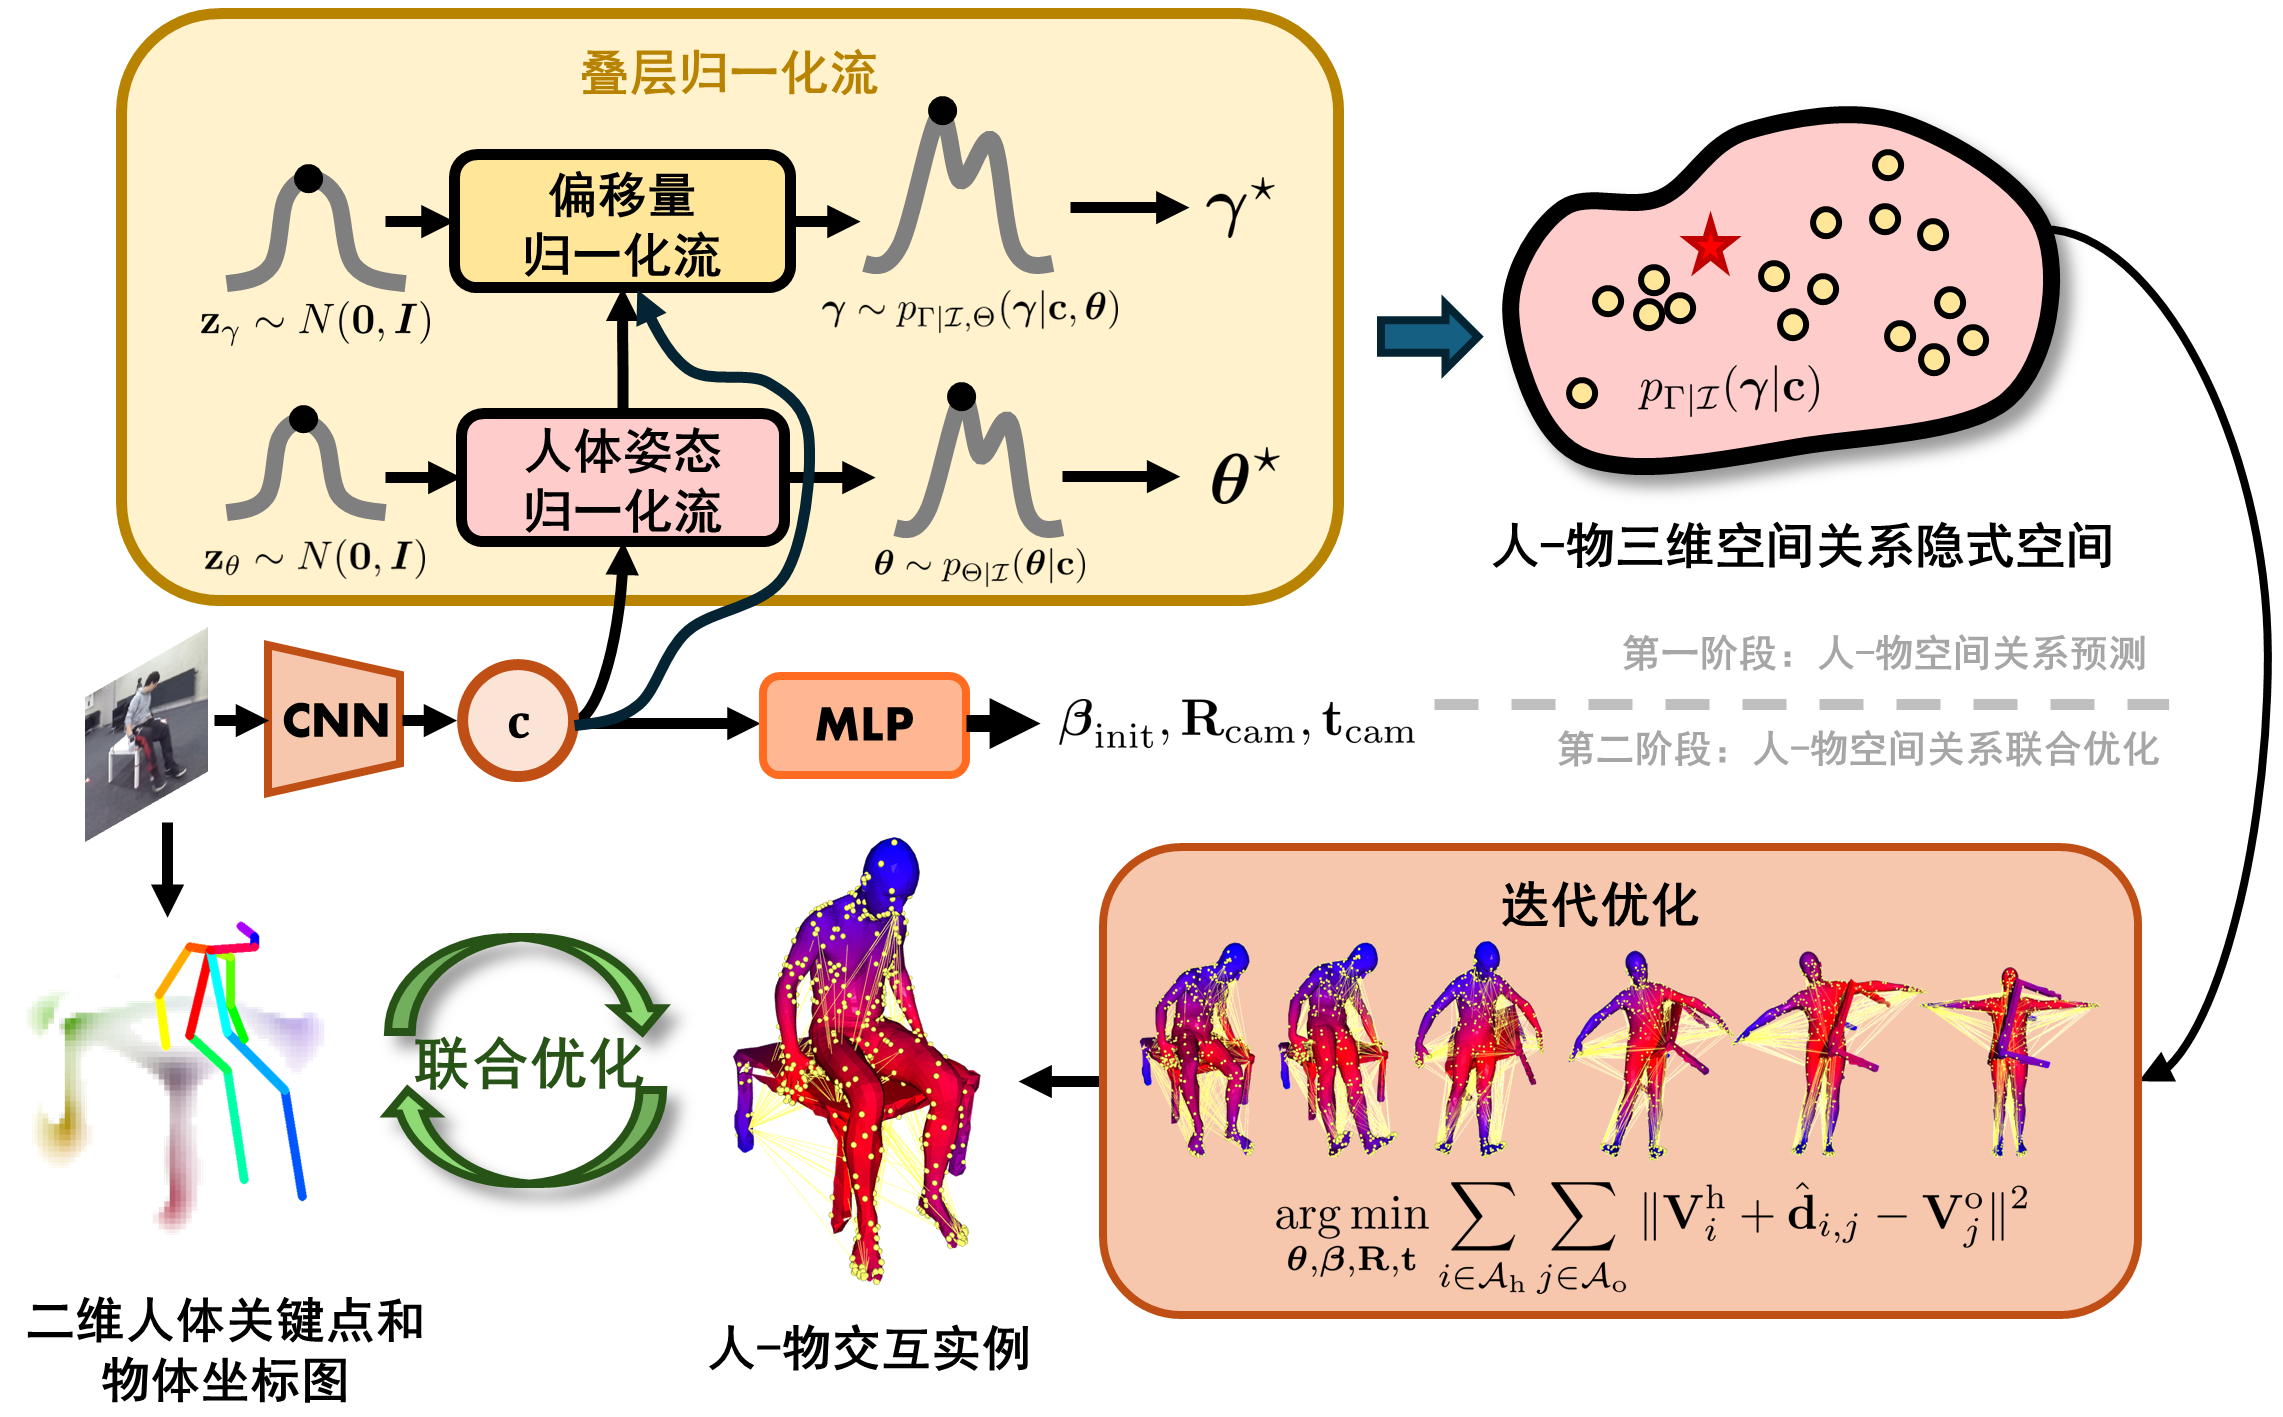
\includegraphics{Img/stackflow}
	\bicaption{基于偏移量的人-物重建算法流程图。}{The main pipeline of the offset-based human-object reconstruction method.}
	\label{fig:stackflow}
\end{figure}

\subsection{人-物空间关系重建网络}
将叠层归一化流集成到人-物空间关系重建网络,如图\ref{fig:stackflow}所示,给定输入图片$\mathbf{I}$,使用卷积网络(convolution neural network)提取视觉特征$\mathbf{c}$,多层感知器(multi-layer perceptron)从视觉特征$\mathbf{c}$提取人体形状参数$\mathbf{\beta}_{\text{init}}$和摄像机的位姿$\mathbf{R}_{\text{cam}},\mathbf{t}_{\text{cam}}$。叠层归一化流从视觉特征$\mathbf{c}$中提取人体姿态概率密度分布$p_{\Theta|I}(\mathbf{\theta}|\mathbf{c})$和人和物体关系的概率密度分布$p_{\Gamma|I,\Theta}(\mathbf{\gamma}|\mathbf{c},\mathbf{\theta})$,在预测阶段,取最高概率似然得到人体姿态的预测结果
\begin{equation}
	\mathbf{\theta}^\star = \mathop{\arg\max}\limits_{\mathbf{\theta}} p_{\Theta|\mathcal{I}}(\mathbf{\theta}) = f_{\mathbf{\theta}}(\mathbf{0}|\mathbf{c}),
\end{equation}
第二个等式成立是由于所选取的归一化流模型的雅可比行列式和$\mathbf{z}_{\mathbf{\theta}}$无关,即式(\ref{eq:theta_log_prob})中雅可比行列式$\left| \det \frac{\partial f_{\mathbf{\theta}}}{\partial \mathbf{z}_{\mathbf{\theta}}} \right|$为一个不取决于$\mathbf{z}_{\mathbf{\theta}}$的常量。同样,人-物三维空间关系的预测结果为
\begin{equation}\label{eq:gamma-prediction}
	\mathbf{\gamma}^\star = \mathop{\arg\max}\limits_{\mathbf{\gamma}} p_{\Gamma|\mathcal{I},\Theta}(\mathbf{\gamma}|\mathbf{c},\mathbf{\theta}^\star) = f_{\mathbf{\gamma}}(\mathbf{0}|\mathbf{c},\mathbf{\theta}^\star).
\end{equation}
使用$\mathbf{\beta}_{\text{init}}$和$\mathbf{\theta}^\star$按照式(\ref{eq:smpl-blending})来初始化人体模型,并得到人体模型表面顶点坐标$\mathbf{V}^{\text{h}}$,固定人体模型顶点坐标,通过下述优化问题求得物体在人体局部坐标系下的位姿,
\begin{eqnarray}
	\mathbf{R}^\star, \mathbf{t}^\star = \mathop{\arg\min}\limits_{\mathbf{R},\mathbf{t}} \sum_{i\in\mathcal{A}_{\text{h}}}\sum_{j\in\mathcal{A}_\text{o}} \| \mathbf{V}_i^\text{h} + \mathbf{d}_{i,j}^\star - \mathbf{V}_j^\text{o} \|^2,
\end{eqnarray}
式中$\mathbf{d}_{i,j}^\star$取自于从$\mathbf{\gamma}^\star$按照式(\ref{eq:reproject-offset})解码出的锚点偏移向量中对应的元素,注意到该优化问题具有闭式解\citep{Choy_2020_CVPR}。

为训练该模型,参照\citep{Kolotouros2021ProbabilisticMF},目标函数为
\begin{equation}
	\mathcal{L}_{\text{train}} = \lambda_{\text{NLL}} \mathcal{L}_{\text{NLL}}^{\text{train}} + \lambda_{\text{exp}} \mathcal{L}_{\text{exp}} + \lambda_{\text{mode}} \mathcal{L}_{\text{mode}} + \lambda_{\text{cam}} \mathcal{L}_{\text{cam}} + \lambda_{\mathbf{\beta}} \mathcal{L}_{\mathbf{\beta}},
\end{equation}
式中,$\lambda$为各个损失的权重,$\mathcal{L}_{\mathbf{\beta}}$为对预测结果$\mathbf{\beta}_{\text{init}}$和标签$\mathbf{\beta}_{\text{gt}}$之间均方误差损失,即
\begin{equation}
	\mathcal{L}_{\mathbf{\beta}} = | \mathbf{\beta}_{\text{init}} - \mathbf{\beta}_{\text{gt}} |_1.
\end{equation}
类似地,$\mathcal{L}_{\text{cam}}$为对摄像机位姿$\mathbf{R}_{\text{cam}}, \mathbf{t}_{\text{cam}}$的损失,使用均方误差计算$\mathbf{R}_{\text{cam}}$的旋转角损失,使用$\ell$-1损失计算$\mathbf{t}_{\text{cam}}$的损失,损失$\mathcal{L}_{\text{NLL}}$为标签$\mathbf{\gamma}_{\text{gt}}$和$\mathbf{\theta}_{\text{gt}}$的负对数似然(negative log-likelihood)损失,具体形式为
\begin{equation}\label{eq:nll-train}
	\mathcal{L}_{\text{NLL}}^{\text{train}} = - \ln p_{\Gamma|\mathcal{I},\Theta}(\mathbf{\gamma}_{\text{gt}}|\mathbf{c}, \mathbf{\theta}_{\text{gt}}) - \ln p_{\Theta|\mathcal{I}}(\mathbf{\theta}_{\text{gt}}|\mathbf{c}).
\end{equation}
损失$\mathcal{L}_{\text{mode}}$为对$\mathbf{\theta}^\star$和$\mathbf{R}^\star, \mathbf{t}^\star$的损失,具体包含对预测结果自身的均方误差损失和人-物关键点的三维坐标损失和二维投影坐标点的损失,而损失$\mathcal{L}_{\text{exp}}$为对样本$\mathbf{\gamma} \sim p_{\Gamma|\mathcal{I},\Theta}$和样本$\mathbf{\theta}\sim p_{\Theta|\mathcal{I}}$的损失,这些损失具体定义参照\citep{Kolotouros2021ProbabilisticMF}。

\subsection{联合优化}
为了使预测的结果能够跟输入图片中人体和物体的二维投影位置保持对齐,使用重投影损失进一步微调预测的结果$\{\mathbf{\beta}, \mathbf{\theta}, \mathbf{R}, \mathbf{t}\}$。记$\mathbf{J}^{\text{3D}}$为人体关键点的三维坐标,$\hat{\mathbf{J}}^{\text{2D}}$为人体二维关键点,这些二维关键点由ViTPose\citep{NEURIPS2022_fbb10d31}提取,人体的重投影损失为
\begin{equation}\label{eq:joint_loss}
	\mathcal{L}_{\mathbf{J}} = \sum_{i=1}^K \| \Pi(\mathbf{J}_i^{\text{3D}}) - \hat{\mathbf{J}}^{\text{2D}} \|^2,
\end{equation}
式中,$K$为人体关键点的个数,$\Pi: \mathbb{R}^3 \to \mathbb{R}^2$为摄像机的投影函数。使用Epro-PnP\citep{Chen_2022_CVPR:epro_pnp}提取物体的三维模型坐标$\mathbf{x}^{\text{3D}}\in \mathbb{R}^{N\times 3}$、二维图片坐标$\mathbf{x}^{\text{2D}}\in\mathbb{R}^{N \times 2}$以及权重$\mathbf{w}^{\text{2D}}\in \mathbb{R}_+^{N\times 2}$,物体的重投影损失计算如下
\begin{equation}\label{eq:coor_reprojection}
	\mathcal{L}_{\text{coor}} = \sum_{i=1}^N \| \mathbf{w}_i^{\text{2D}} \circ (\Pi(\mathbf{R}\mathbf{x}_i^{\text{3D}} + \mathbf{t}) - \mathbf{x}_i^{\text{2D}}) \|_1.
\end{equation}
除重投影损失,为了限制人和物体之间的关系在优化过程中不被打乱,增加对人和物体之间空间关系基于偏移量的损失,其定义如下
\begin{equation}\label{eq:nll-optim}
	\mathcal{L}_{\text{NLL}}^{\text{optim}} = - \ln p_{\Gamma|I,\Theta}(\mathbf{\gamma}|\mathbf{c}, \mathbf{\theta}) - \ln p_{\Theta|I}(\mathbf{\theta}|\mathbf{c}).
\end{equation}
注意式(\ref{eq:nll-train})和式(\ref{eq:nll-optim})的差异,式(\ref{eq:nll-train})是在训练中的损失,其中可变参数为归一化流模型StackFLOW的参数,而在联合优化过程中,重建模型StackFLOW内部参数固定,可变参数为$\{\mathbf{\beta}, \mathbf{\theta}, R, \mathbf{t}\}$。将以上三个优化函数合并得到总优化目标函数
\begin{equation}
	\mathcal{L}_{\text{optim}} = \lambda_{\mathbf{J}} \mathcal{L}_{\mathbf{J}} + \lambda_{\text{coor}} \mathcal{L}_{\text{coor}} + \lambda_{\text{NLL}} \mathcal{L}_{\text{NLL}}^{\text{optim}},
\end{equation}
式中,$\lambda_{\mathbf{J}},\lambda_{\text{coor}},\lambda_{\text{NLL}}$为优化损失对应的权重。

\section{实验结果及分析}\label{sec:exp-stackflow}

\subsection{数据集与评价指标}
为分析本章所提出的算法在人-物重建人物上的性能,在BEHAVE数据集上开展实验。BEHAVE数据集\citep{Bhatnagar_2022_CVPR:BEHAVE}是一个包含人体和物体交互的数据集,该数据集由多摄像机动捕系统所构建,包含了人和常见的20个物体的交互,数据集中共包含由4架Kinect RGB-D摄像机所拍摄的帧率为30的视频序列,并对每一张图片提供了SMPL的伪标签、物体6D位姿标签以及摄像机的位姿和标定参数。在实验中,使用官方所提供的划分,217个视频序列用于训练,82个序列用于测试。由于本章所提出的方法对人-物的静态重建算法,在测试时,测试图片的帧率在1FPS,即对视频序列中每1秒抽取一张图片测试,计算每张图片的倒角距离,最后取平均。除BEHAVE数据集外,还在InterCap数据集上进行实验。InterCap也是一个全身人体和物体交互的三维数据集,包含大概4M张包含10个人和10个物体的交互的图片,类似于BEHAVE数据集,InterCap数据集也提供了SMPL的伪标签和物体的6D位姿。由于官方没有划分测试集和训练集,实验中随机选取20\%的序列用于测试,剩余用于训练,在这种划分下,训练集包含326, 955张图片,而测试集包含73, 541张图片。

在性能评估方面,主要使用重建的三维网格模型和标签之间的倒角距离(chamfer distance)来衡量重建精度,在计算倒角距离之前,从重建的人体和物体网格模型表面采样出10000个点,同样 从标签网格模型中采样出10000个点,使用最优普氏对齐(optimal  Procrustes alignment)将重建网格模型表面采用出的点云和标签网格模型的点云进行对齐,计算这两个点云之间的倒角距离,人体的倒角距离和物体的倒角距离分别汇报。除倒角距离外,使用模型的GFLOPs、参数量以及模型使用处理一张图片的平均时间对比模型的计算复杂度和空间复杂度。

\subsection{实验参数设置}
人-物关系建模方面,人体模型中每个身体部位采样32个点,得到$22 \times 32 = 704$个人体锚点,物体模型采样64个点,主成分分析时提取前32个主成分构成隐式空间的基向量。网络结构方面,使用ResNet-50作为图片的特征提取器,归一化流模型$f_{\text{SMPL}}$和$f_{\text{object}}$均由8层归一化层、可逆线性层、解耦层构成,网络内部各个超参数见本文所附代码。在训练该网络时,在BEHAVE数据集上使用Adam优化器训练10轮,在第7轮时学习率从0.0001缩减10倍。训练过程中,使用了背景增强策略,随机更换输入图片的背景(除人和物体以外的区域),使用背景增强后,网络收敛速度和重建结果有很明显的提升。在后优化过程中,人的重投影损失权重$\lambda_{\mathbf{J}}=0.1$,物体的重投影损失权重$\lambda_{\text{coor}}=10$,偏移量的损失权重$\lambda_{\text{NLL}}=1$,优化分成两个阶段,每个阶段迭代500步,初始优化器的学习率为0.05,第一阶段过后学习降为原来的十分之一。

\subsection{自由视角数据增强}
为了进一步提高模型在测试集合上的泛化性能,使用了自由视角增强的策略来生成新的图像以扩充原有数据集。首先,对于数据集中每个样本,使用在CAPE数据集\citep{Pons-Moll:Siggraph2017, Ma2019LearningTD}训练的MetaAvatar\citep{Wang2021MetaAvatarLA}来生成给定人体姿态$\mathbf{\theta}$参数后对应的着装后的人体网格模型,将该模型和带有纹理的物体网格模型放置在同一坐标系下,为后一步渲染做准备,这里人体网格模型和物体网格模型之间的位姿由$\{\mathbf{R}, \mathbf{t}\}$确定。在渲染过程中,通过改变摄像机的位姿来生成包含各种人-物遮挡情况的图片,所生成的图片如图\ref{fig:view_aug}所示。最终,对数据集中的每一个人-物交互类型生成了12张从不同角度观测的图片,这些生成的图片作为训练模型的一个辅助的扩充数据集。

\begin{figure}[!htbp]
	\centering
	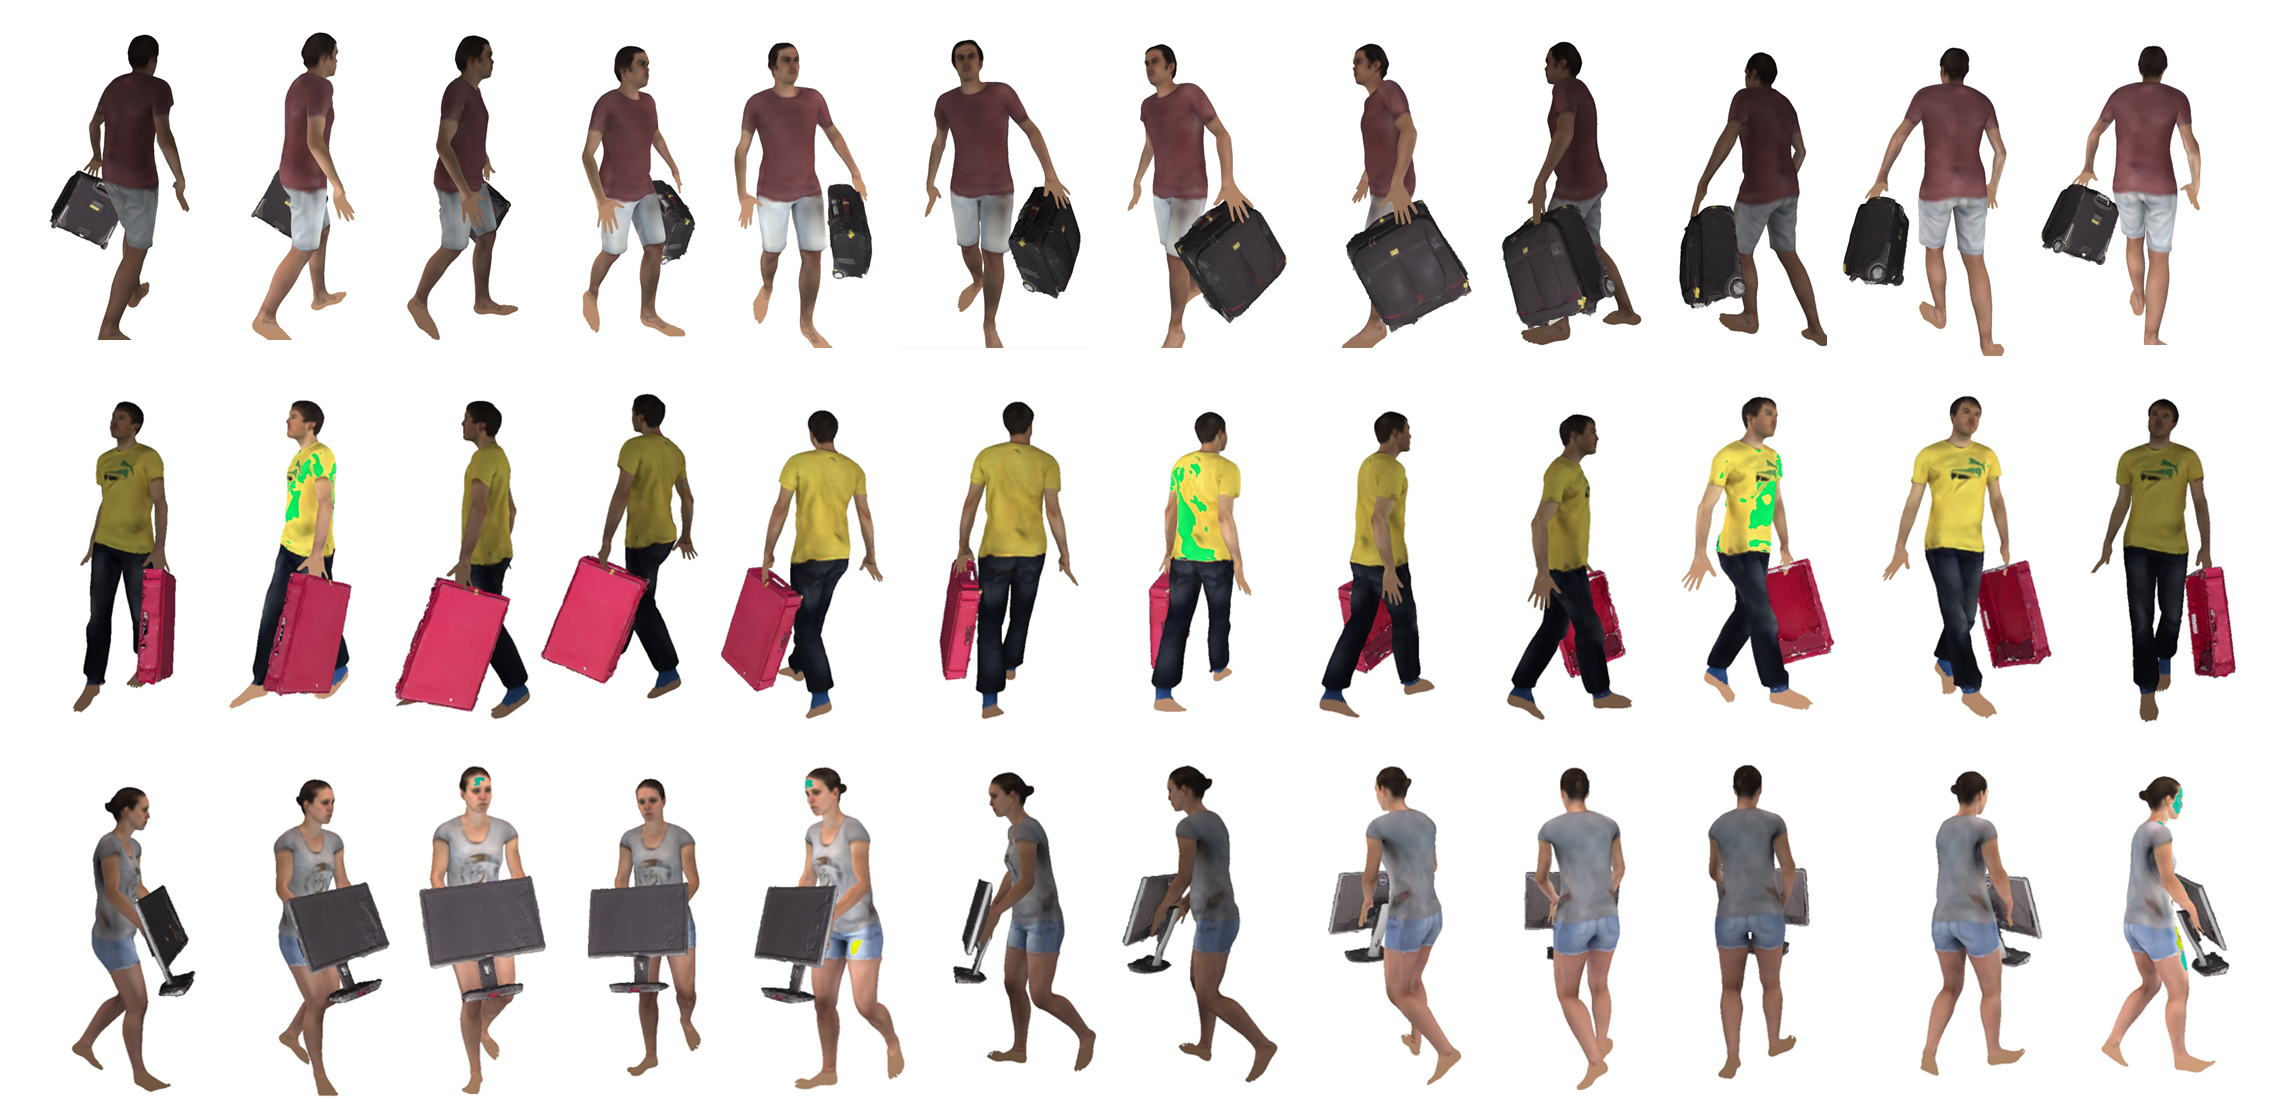
\includegraphics{Img/view_aug}
	\bicaption{\centering{使用自由视角数据增强的方式所生成的各个视角下的图片}}{\centering{In this figures, we show the fake images generated by our free-viewport data augmentation from different view.}}
	\label{fig:view_aug}
\end{figure}

\subsection{总体性能分析}
\paragraph{定量分析}
将本章所提出的方法和当前两大方法PHOSA和CHORE在BEHAVE数据集和InterCap数据集上进行了比较。PHOSA\citep{zhang2020phosa}是一种基于优化的方法,该方法在优化过程中,利用人为预先构建的先验知识来将人和物体相接触的地方拉近;CHORE\citep{xie2022chore}是基于学习的方法,该方法从图片中提取人-物交互的隐式距离场,在优化过程中将人体和物体的网格模型拟合到该隐式距离场中。在表\ref{tab:stackflow_behave_performance}中,从运行效率和重建精度维度和这两个方法进行了对比。在模型参数量方面,由于PHOSA是一种基于纯优化的方法,PHOSA所需要的模型参数量为0,本章所提出的方法使用到ResNet-50因而模型的参数量会远高于CHORE。在模型的计算复杂度方面,本章所提出的方法要远远优于CHORE,这种差距在实际的运行时间对比更加明显,本章使用预测-优化的框架,在预测阶段得到一个好的初始化结果,因而在后优化阶段只需要很少的迭代次数,并且在后优化阶段本章所提出的优化目标函数计算效率要更加高效,而CHORE使用到隐式向量场,为得到更加精确的结果,需要采样出很多点来逼近表面,需要更多的计算量,本章所提出的方法在后优化过程中需要最大化人-物空间关系的概率后验密度,每迭代一次都需要使用叠层归一化流来预测出当前结果的概率密度,因此优化一张图片所需要的时间稍高于PHOSA。在重建角度方面,本章所提出的方法的优于CHORE,在没有使用后优化的前提下,本章所提出的方法已经达到不错的精度,在加入后优化后,全方位超越其它两个方法。总之,本文所提出的方法与之前的方法相比,具有更高的重建精度和很快的运行效率。

\begin{table}[!htbp]
	\bicaption{\centering{不同方法在BEHAVE数据集和InterCap数据集上的性能对比。}}{\centering{Performance comparison of different methods on BEHAVE dataset and InterCap dataset.}}
	\label{tab:stackflow_behave_performance}
	\centering
	\footnotesize
	\setlength{\tabcolsep}{4pt}
	\renewcommand{\arraystretch}{1.2}
	\begin{tabular}{lccccccc}
		\toprule
		\multirow{2}{*}{方法} & \multirow{2}{*}{参数量(M)} & \multirow{2}{*}{GFLOPs} & \multirow{2}{*}{时间(s)} & \multicolumn{2}{c}{BEHAVE} & \multicolumn{2}{c}{InterCap} \\
		\cline{5-8}
		& & & & 人体 & 物体 & 人体 & 物体 \\
		\hline
		PHOSA & - & - & 14.23 & 12.86 & 26.90 & 6.06 & 14.81 \\
		CHORE & \textbf{18.19} & 396.39 & 366.04 & 5.54 & 10.12 & 6.86 & 15.49 \\
		StackFLOW & 77.02 & \textbf{5.50} & \textbf{1.15} & 5.10 & 14.01 & 4.96 & 11.53 \\
		StackFLOW (+后优化) & 77.02 & \textbf{5.50} & 43.39 & \textbf{4.79} & \textbf{9.12} & \textbf{4.42} & \textbf{8.04} \\
		\bottomrule
		\multicolumn{6}{l}{注:加粗字体为最优结果。}
	\end{tabular}
\end{table}

进一步,在实验中将本章所提出的算法在BEHAVE数据集上进行全量图片测试,评测标准参考VisTracker\citep{bhatnagar22behave}。结果如表\ref{tab:stackflow_behave_performance_seq}所示,可以发现由于本章所提出的方法使用ProHMR来提取人体位姿,本章所提出方法在人体重建精度最优,而物体重建的精度仅次于VisTracker,注意到本文没有对视频中物体的运动轨迹上做出特定的限制,所以在物体上的效果略低于VisTracker。整体上再次印证了本章所提出算法的有效性。

\begin{table}[!htbp]
	\bicaption{\centering{不同方法在BEHAVE数据集的性能对比。}}{\centering{Performance comparison of different methods on BEHAVE dataset.}}
	\label{tab:stackflow_behave_performance_seq}
	\centering
	\footnotesize
	\setlength{\tabcolsep}{4pt}
	\renewcommand{\arraystretch}{1.2}
	\begin{tabular}{lccccc}
		\toprule
		\multirow{2}{*}{方法} & \multirow{2}{*}{后优化} & \multicolumn{2}{c}{Align $w$ = 1} & \multicolumn{2}{c}{Align $w$ = 10} \\
		\cline{3-6}
		& & 人体 & 物体 & 人体 & 物体 \\
		\hline
		CHORE & \Checkmark & 5.55 & 10.02 & 18.33 & 20.32 \\
		VisTracker & \Checkmark & 5.25 & \textbf{8.04} & 7.81 & \textbf{8.49} \\
		StackFLOW & \XSolidBrush & \textbf{4.42} & 10.87 & 5.23 & 11.64 \\
		StackFLOW & \Checkmark & 4.39 & 8.57 & \textbf{4.98} & 8.94 \\
		\bottomrule
		\multicolumn{6}{l}{注:加粗字体为最优结果。}
	\end{tabular}
\end{table}


\paragraph{定性分析}
在图\ref{fig:comparison-on-intercap}中,对比了单独重建和带有偏移量重建的结果,单独重建表示没有对人体和物体之间的位姿进行约束,而偏移量重建表示使用偏移量约束人体和物体之间的位姿,从图中可以看出引入偏移量后能够明显约束人体和物体之间的相对位姿,单独重建虽然能够在输入视角和输入图片保持对齐,但在侧面视角人体和物体之间存在较大误差,而加入偏移量约束人体和物体之间的位姿之后能够生成更加合理、自然的结果。
在图\ref{fig:comparison-with-chore}中,本章所提出的方法和CHORE针对严重遮挡的情况进行了定性对比,图中使用红色的圈圈出重建不合理的部位。从图中可以看出,即使人体某些部位被物体遮挡,或者物体被人体严重遮挡,本章所提出的方法仍然可以从可见的人体或者物体部分猜测出被遮挡部位的位姿,而CHORE对遮挡情况鲁棒性不如本章所提出的方法。对遮挡情况鲁棒性得益于本章所提出的基于偏移量的表示,在基于偏移量的表示中,使用人和物体之间的偏移量对人和物体统一建模,因而在预测阶段中,即使被遮挡后,被遮挡的部位的位姿仍然可以通过偏移量从可见的部位推测出。

\begin{figure}[!htbp]
	\centering
	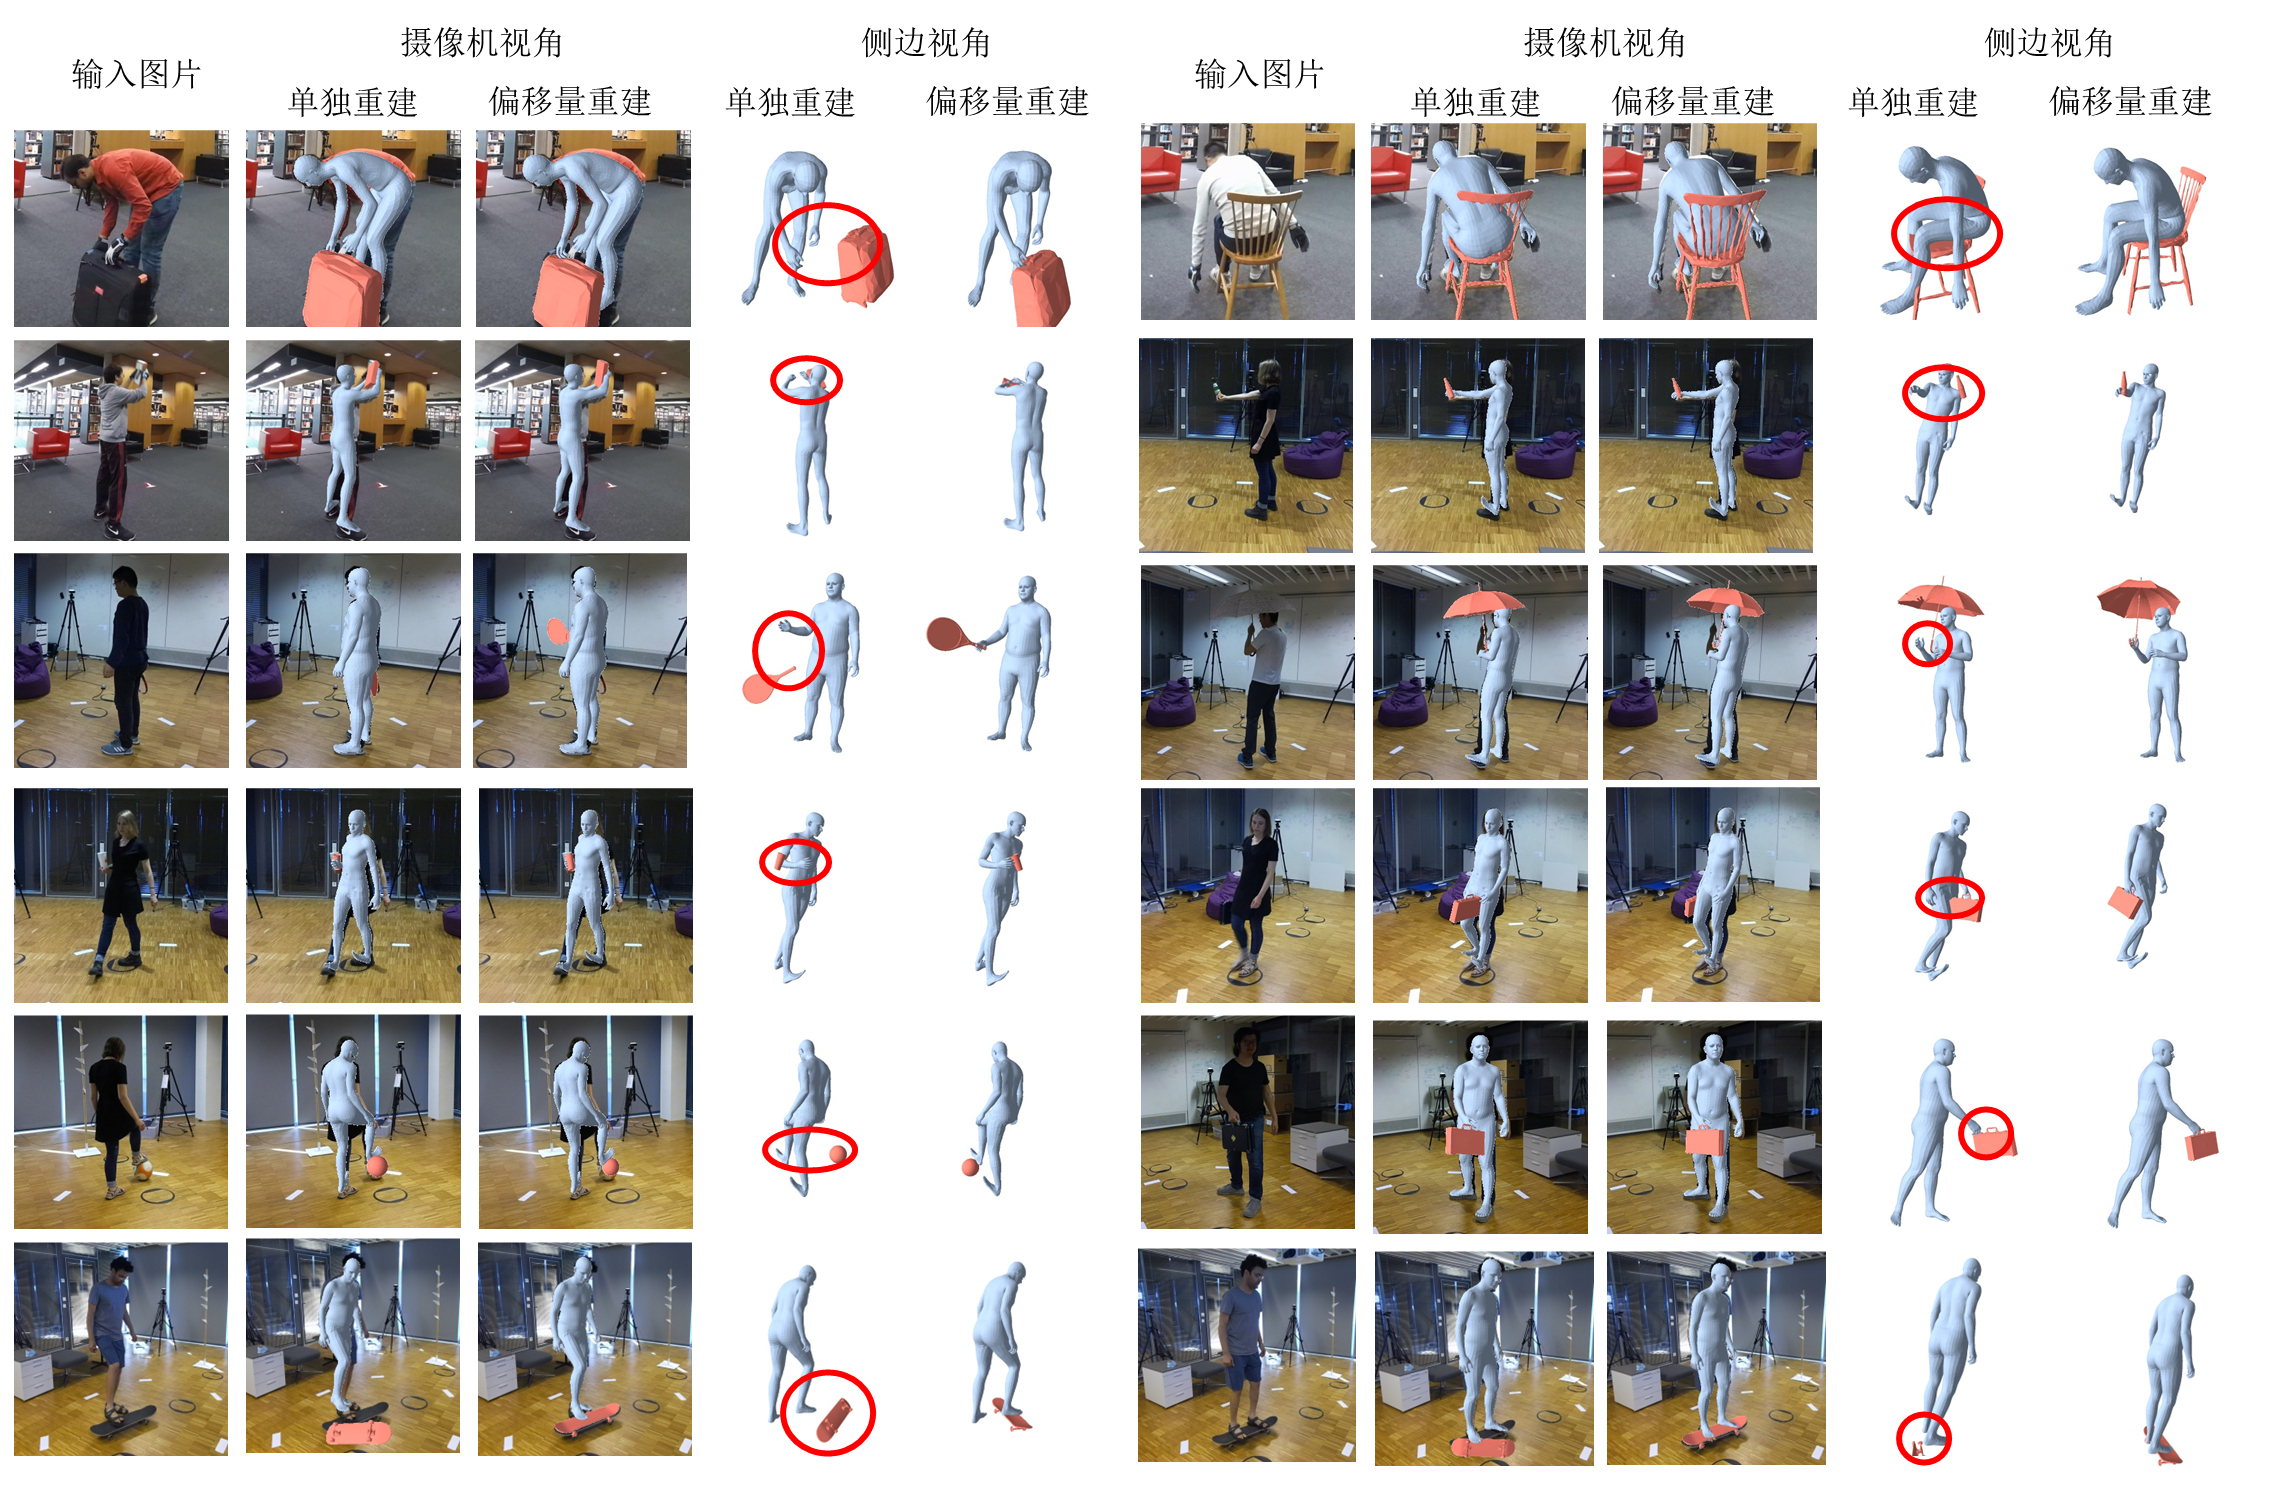
\includegraphics{Img/comparison_intercap}
	\bicaption{本章所提出的方法在InterCap数据集上的定性对比。}{Quantization comparison on InterCap dataset.}
	\label{fig:comparison-on-intercap}
\end{figure}

\begin{figure}[htbp]
	\centering
	\includegraphics{Img/comparison_stackflow}
	\bicaption{本章所提出的方法和CHORE在BEHAVE数据集上的定性对比。}{Quantization comparison between our method and CHORE on BEHAVE dataset.}
	\label{fig:comparison-with-chore}
\end{figure}

\subsection{消融实验}
为验证提出的所基于偏移量表征的对人-物空间关系编码的信息保真度,设计以下实验。对每一个人-物交互实例按照章节\ref{sec:offset-representation}提取人-物空间关系编码$\mathbf{\gamma}$,使用反投影(式(\ref{eq:reproject-offset}))得到偏移量$\mathbf{d}$,之后从$\mathbf{d}$中按照式(\ref{eq:recon_from_offset})重构出参数$\{\mathbf{\beta}, \mathbf{\theta}, \mathbf{R}, \mathbf{t}\}$,人体模型表面顶点$\mathbf{P}^{\text{h}}$从$\mathbf{\beta}, \mathbf{\theta}$中重构出,而物体表面顶点$\mathbf{P}^{\text{o}}$从$\mathbf{R}, \mathbf{t}$重构出,计算重构出的参数和标签之间的$\ell$-1距离,得到表\ref{tab:ablation_anchor_num}中的结果。从表中可以看出,基于偏移量对信息保存完整,重构出的人的顶点误差和物的顶点平均误差均在1cm内,$\mathbf{\gamma}$的维度对重建误差具有较大的影响,高纬度的$\mathbf{\gamma}$对信息保存更完整,但高纬度$\mathbf{\gamma}$会带来额外的计算开销。人体锚点数量$m$和物体锚点数量$n$对重建结果影响并不明显,这是由于物体网格模型和人体网格模型中顶点存在一定的相互约束,即使使用少量的锚点也能得到和使用大量锚点相媲及的重建精度。

\begin{table}[!htbp]
	\bicaption{\centering{人-物网格模型表面锚点数量和隐式空间的维度对重建误差的影响。}}{\centering{The influence of the number of the human anchors, object anchors and the dimension of the latent relation space to the reconstruction accuracy.}}
	\label{tab:ablation_anchor_num}
	\centering
	\footnotesize
	\setlength{\tabcolsep}{4pt}
	\renewcommand{\arraystretch}{1.2}
	\begin{tabular}{c|c|cccc|cccc|cccc}
		\toprule
		\multirow{3}{*}{超参数} & $k$ & \multicolumn{4}{c}{32} & \multicolumn{4}{c}{64} & \multicolumn{4}{c}{128} \\
		\cline{2-14}
		& $m$ & 88 & 176 & 352 & 704 & 88 & 176 & 352 & 704 & 88 & 176 & 352 & 704 \\
		& $n$ & 8 & 16 & 32 & 64 & 8 & 16 & 32 & 64 & 8 & 16 & 32 & 64 \\
		\hline
		\multirow{7}{*}{重建误差} & $\mathbf{\beta}$ & 0.554 & 0.567 & 0.596 & 0.596 & 0.359 & 0.321 & 0.316 & 0.319 & 0.297 & 0.243 & 0.230 & 0.235 \\
		& $\mathbf{\theta}$ & 0.138 & 0.121 & 0.117 & 0.119 & 0.090 & 0.070 & 0.063 & 0.067 & 0.064 & 0.042 & 0.037 & 0.044 \\
		& $\mathbf{R}$ & 0.044 & 0.039 & 0.018 & 0.018 & 0.060 & 0.025 & 0.022 & 0.018 & 0.050 & 0.044 & 0.033 & 0.020 \\
		& $\mathbf{t}$ & 0.006 & 0.006 & 0.005 & 0.006 & 0.003 & 0.002 & 0.002 & 0.002 & 0.003 & 0.002 & 0.001 & 0.001 \\
		& $\mathbf{P}^{\text{h}}$ & 0.009 & 0.009 & 0.009 & 0.009 & 0.003 & 0.003 & 0.002 & 0.002 & 0.002 & 0.001 & 0.001 & 0.002 \\
		& $\mathbf{P}^{\text{o}}$ & 0.008 & 0.008 & 0.006 & 0.006 & 0.005 & 0.003 & 0.003 & 0.002 & 0.005 & 0.004 & 0.003 & 0.002 \\
		& $\mathbf{d}$ & 0.008 & 0.007 & 0.007 & 0.007 & 0.002 & 0.002 & 0.002 & 0.002 & 0.000 & 0.000 & 0.001 & 0.001 \\
		\bottomrule
	\end{tabular}
\end{table}

进一步,在表\ref{tab:ablation_representation}中,对比了隐向量$\mathbf{\gamma}$维度、人体锚点数量$m$和物体锚点数量$n$在实际应用到重建任务中后对重建精度的影响。从表中可以看出,选取的锚点数量越多重建精度越高,但提升微乎其微。在$\mathbf{\gamma}$使用较大的维度后,结果提升不如期望,这是由于较高的维度会带来模型参数的变多,进而影响训练过程,从而在测试集的表现不如预期。

\begin{table}[!htbp]
	\bicaption{\centering{隐向量$\mathbf{\gamma}$维度、人体锚点数量$m$和物体锚点数量$n$对重建结果的影响。}}{\centering{The effectiveness of the number of the dimension of $\mathbf{\gamma}$, $m$ and $n$ to the reconstruction accuracy.}}
	\label{tab:ablation_representation}
	\centering
	\footnotesize
	\setlength{\tabcolsep}{4pt}
	\renewcommand{\arraystretch}{1.2}
	\begin{tabular}{c|c|ccc|c|c}
		\toprule
		\multirow{3}{*}{超参数} & $k$ & \multicolumn{3}{c|}{32} & 64 & 128 \\
		\cline{2-7}
		& $m$ & 176 & 352 & 704 & 704 & 704 \\
		& $n$ & 16 & 32 & 64 & 64 & 64 \\
		\hline
		\multirow{2}{*}{重建误差} & 人体 & 4.95 & 4.88 & 4.79 & \textbf{4.71} & 4.73 \\
		& 物体 & 9.47 & 9.32 & \textbf{9.12} & 9.87 & 10.88 \\
		\bottomrule
		\multicolumn{6}{l}{注:加粗字体为最优结果。}
	\end{tabular}
\end{table}

在表\ref{tab:ablation_loss}中,对比了联合优化中各个损失对重建结果的影响,其中$\mathcal{L}_{\text{SMPL}}$是对于人体的损失,具体包含人体关键点的重投影损失,即式(\ref{eq:joint_loss})中的$\mathcal{L}_{\mathbf{J}}$,还包括式(\ref{eq:nll-optim})中的对人体姿态的负对数似然$-\ln p_{\Theta|I}(\mathbf{\theta}|\mathbf{c})$的损失。损失$\mathcal{L}_{\text{object}}$是物体的坐标重投影损失,即式(\ref{eq:coor_reprojection})中的$\mathcal{L}_{\text{coor}}$。$\mathcal{L}_{\text{offset}}$是对人和物体之间偏移量的损失即式(\ref{eq:nll-optim})中人-物关系的负对数似然$ - \ln p_{\Gamma|I,\Theta}(\mathbf{\gamma}|\mathbf{c}, \mathbf{\theta})$。人体和物体的重建误差使用和标签的倒角距离衡量,从表中结果可以看出,这三类损失均对重建精度有重要影响,缺一不可,只有共同作用才联合优化上,才能达到最优秀的重建精度。

\begin{table}[!htbp]
	\bicaption{联合优化过程中各个损失对重建结果的影响。}{The effectiveness of different optimization losses on the reconstruction accuracy.}
	\label{tab:ablation_loss}
	\centering
	\footnotesize
	\setlength{\tabcolsep}{4pt}
	\renewcommand{\arraystretch}{1.2}
	\begin{tabular}{ccc|cc}
		\toprule
		\multirow{2}{*}{$\mathcal{L}_{\text{SMPL}}$} & \multirow{2}{*}{$\mathcal{L}_{\text{object}}$} & \multirow{2}{*}{$\mathcal{L}_{\text{offset}}$} & \multicolumn{2}{c}{重建误差} \\
		\cline{4-5}
		&&& 人体 & 物体 \\
		\hline
		\XSolidBrush & \Checkmark & \Checkmark & 8.81 & 16.42 \\
		\Checkmark & \XSolidBrush & \Checkmark & 5.22 & 13.84 \\
		\Checkmark & \Checkmark & \XSolidBrush & 5.24 & 16.95 \\
		\Checkmark & \Checkmark & \Checkmark & \textbf{4.79} & \textbf{9.12} \\
		\bottomrule
		\multicolumn{5}{l}{注:加粗字体为最优结果。}
	\end{tabular}
\end{table}

在表\ref{tab:ablation_augment}中,对比了在使用不同比例的增强数据集对重建结果的影响,表中$\alpha$是增强数据集中用于训练的比例,使用全部的增强数据集训练的模型达到了最高的重建精度(表\ref{tab:ablation_augment}中最后一行),注意到使用全部增强数据和使用一半增强数据的重建指标限差微乎其微,这说明合适的增强数据的比例在0.5-1之间,在生成增强数据集的过程中,摄像机环绕人体一圈,每隔角度$360^\circ / 12 = 30^\circ$渲染一张图片,而增强数据集的比例$0.5$对应于间隔角度为$60^\circ$,这说明在生成数据集时合适的角度为$60^\circ$。

\begin{table}[!htbp]
	\bicaption{\centering{使用不同比例的增强数据对重建结果的影响。}}{\centering{The impact of different fractions of augmentated dataset on the reconstruction accuracy.}}
	\label{tab:ablation_augment}
	\centering
	\footnotesize
	\setlength{\tabcolsep}{4pt}
	\renewcommand{\arraystretch}{1.2}
	\begin{tabular}{c|cccccc}
		\toprule
		$\alpha$ & 0.00 & 0.17 & 0.25 & 0.33 & 0.50 & 1.00 \\
		\hline
		人体 & 4.60 & 4.39 & 4.40 & 4.37 & \textbf{4.33} & \textbf{4.33} \\
		物体 & 9.83 & 9.11 & 9.14 & 9.03 & 8.88 & \textbf{8.87} \\
		\bottomrule
		\multicolumn{6}{l}{注:加粗字体为最优结果。}
	\end{tabular}
\end{table}

\subsection{单人多物交互拓展}
虽然在实验中,本章所提出的使用偏移量来调节人体和物体之间的空间关系的方法是应用于单人单物场景,但本章所提出的算法可以拓展对单人多物的场景中,在单人多物场景中,人的位姿受与之交互的各种物体约束,将多个物体对人体的偏移量同时作用在人体上来共同优化。在图\ref{fig:stackflow_multi_object}中展示了本章算法应用到单人多物场景中的重建结果。

\begin{figure}[htbp]
	\centering
	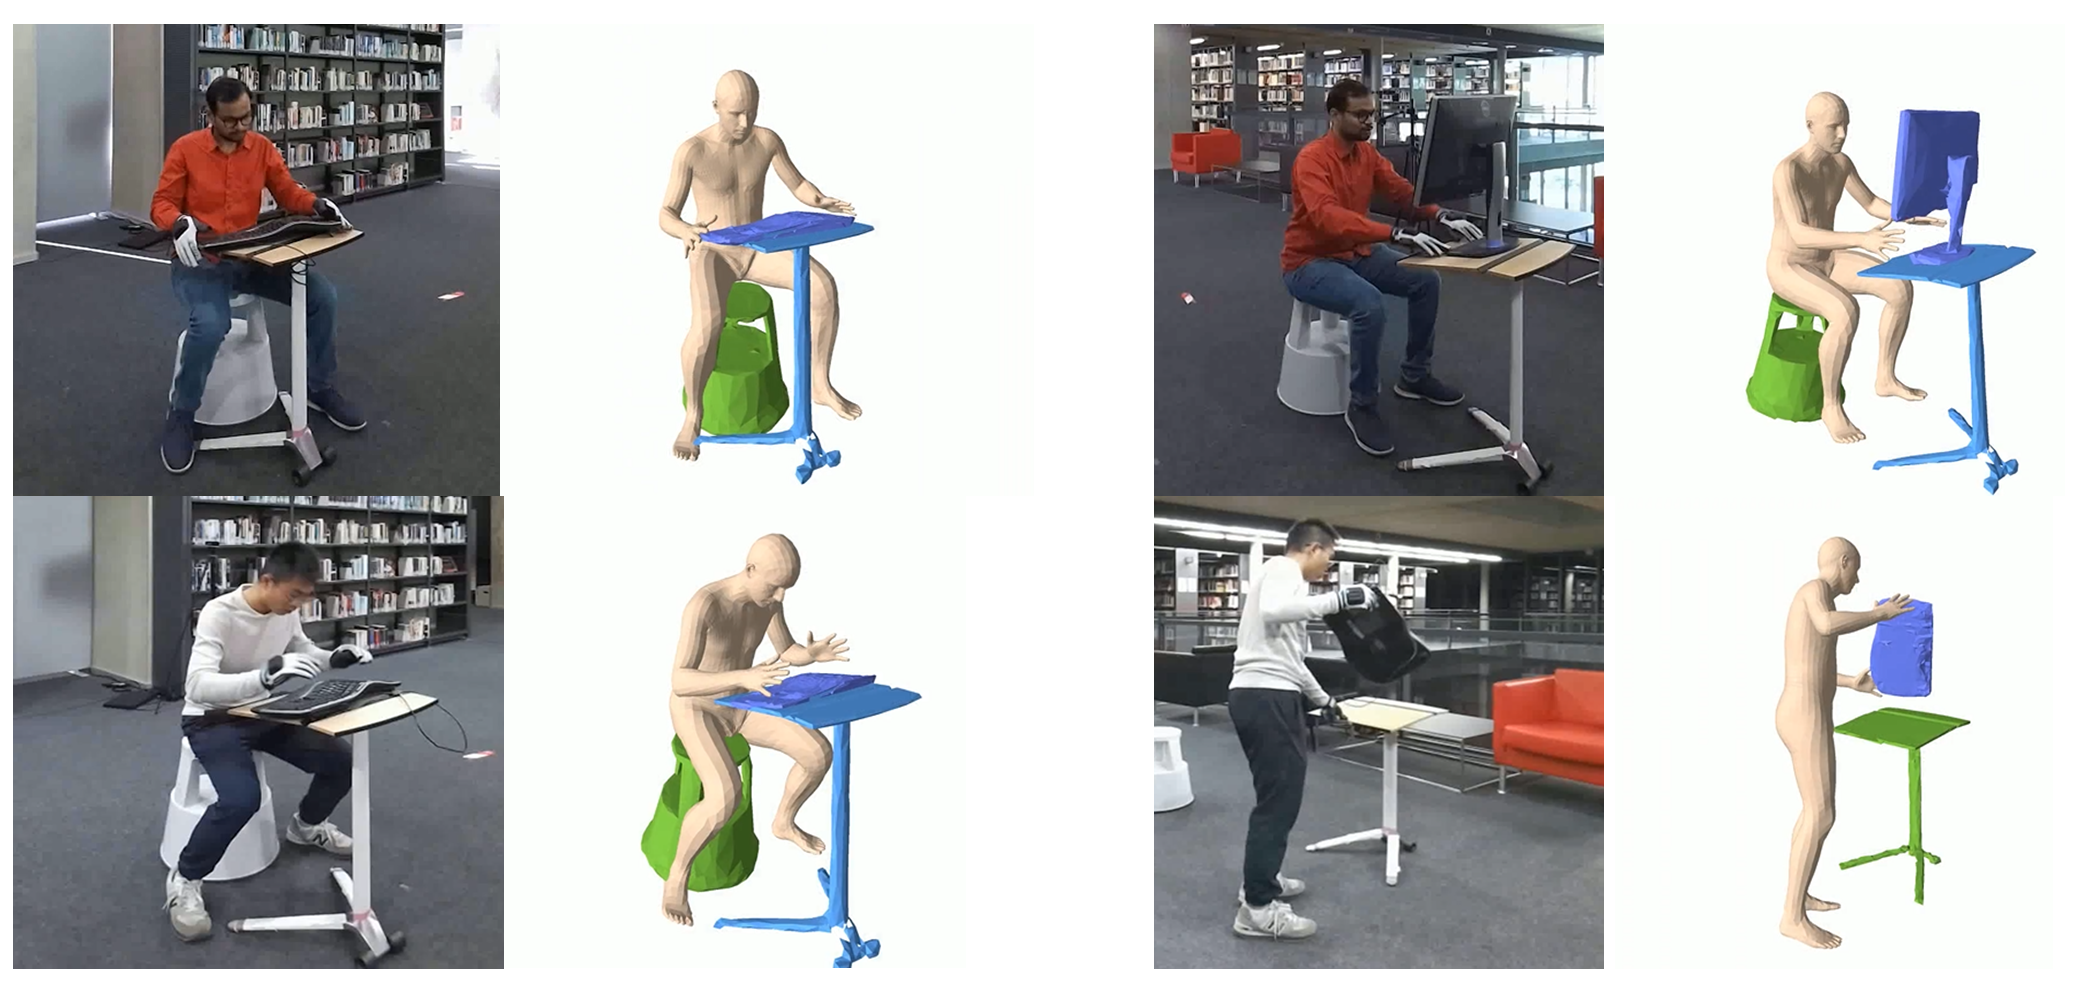
\includegraphics{Img/stackflow_multi_object}
	\bicaption{\centering{StackFLOW应用在单人多物场景中的重建结果。}}{\centering{The qualitative results of the StackFLOW applied to the interaction between single-person and multi-object.}}
	\label{fig:stackflow_multi_object}
\end{figure}

\section{本章小结}
本章提出了一种基于人-物偏移量对人和物体之间空间关系的刻画方式,并将该刻画方式应用在人-物重建问题上。通过计算人和物体之间偏移量,更加准确地描述人和物体之间的相对位置关系,这种刻画方式的优势在于可以将人体和物体用同一个量描述,从而更加方便进行对人-物之间的空间关系的分析和建模。为了将该基于偏移量刻画方式应用到人-物重建问题上,本章还给出了一种预测-优化的两阶段重建算法。在预测阶段,使用叠层归一化流模型预测给定图片的人-物空间关系的后验分布,在后优化阶段,结合重投影损失和该后验分布的损失微调结果。在BEHAVE数据集上的实验结果证明了该方法的有效性,该方法和基于隐式向量场或者基于接触面的方法相比具有更高的重建精度和运行效率,并且对于严重遮挡的情况具有更高的鲁棒性。

尽管本章所提出的方法在BEHAVE数据集取得了很不错的结果,但仍然存在一些局限性。首先,本章所提出的方法是建立在物体网格模型已知的前提下,该方法只能应用于包含指定物体的人-物重建,在这种限制导致该方法不能应用到大多数场景中。其次,该方法在构建人和物体空间关系的隐式表达时,需要预先在人体和物体网格模型选择锚点并且进行PCA降维处理,这种以离线形式所构建的隐式人-物交互关系空间不能在后续动态调整,不是端到端的方式。最后,本章所提出的算法泛化能力较差,该方法由于将图片作为一种条件输入到叠层归一化流中,因此对于训练集差距较大的自然场景中的图片,该方法泛化能力较差。

针对这些局限性,未来的工作可以探索以下几个方向进行改进和优化:
\begin{itemize}
	\item 扩展到无网格模型的场景:可以考虑将方法扩展到无网格模型的情况下,通过学习更加通用的人体和物体表示来解决这个问题。这样可以使方法更具有普适性,适用于更广泛的场景。
	\item 端到端学习:将人体和物体之间的空间关系的表达方式改为端到端学习,可以更好地动态调整人-物交互空间表示,提高方法的灵活性和准确性。
	\item 提高泛化性能:可以通过引入更多的数据增强技术,或者修改网络结构,使其更好地适应不同风格和场景的图片,从而提高方法的泛化能力。
\end{itemize}
通过以上不断的改进和优化,可以使基于人-物偏移量的空间关系刻画方法在人-物重建问题上取得更好的效果,并且在实际应用中发挥更大的作用。